\chapter{PENGUJIAN DAN ANALISIS}
\label{chap:pengujiananalisis}

% Ubah bagian-bagian berikut dengan isi dari pengujian dan analisis

Pada bab ini akan membahas tentang pengujian sistem perencanaan gerakan mobil otonom dengan menggunakan algoritma DQN. Kemudian, akan dilakukan analisis terhadap hasil simulasi sistem
perencanaan gerakan mobil otonom yang telah dirancang.

\section{Training DQN}
\label{sec:training_dqn}
Training algoritma DQN dilakukan dengan menggunakan hardware berikut:
\begin{table}[H]
	\begin{tabular}{ll}
		\textbf{CPU}  & Intel Core i5              \\
		\textbf{GPU}  & Nvidia GTX 1060 - 6GB VRAM \\
		\textbf{RAM}  & 8GB                        \\
		\textbf{Disk} & 256GB SSD M.2              \\
		\textbf{OS}   & Windows 10                
	\end{tabular}
\caption{\textit{Hardware} yang digunakan untuk \textit{training}.}
\label{tb:hardwaresetup}
\end{table}

\textit{Training} dilakukan dengan mesin lokal menggunakan GPU. Lingkungan \textit{software} \textit{machine learning} yang digunakan pada saat \textit{training }berupa:

\begin{table}[H]
	\begin{tabular}{ll}
		\textbf{Software}  & \textbf{Version}              \\
		tensorflow-gpu  & 1.13.1	\\
		keras  & 2.2.5					\\
		h5py & 3.1              \\
		python & 3.7.9              \\
	\end{tabular}
	\caption{Lingkungan software yang digunakan untuk learning.}
	\label{tb:softwaresetup}
\end{table}


Hasil dari proses \textit{training} tersebut adalah model jaringan DQN yang merepresentasikan sistem perencanaan gerakan mobil otonom. Model tersebut disimpan dalam sebuah file berformat .model yang selanjutnya dapat divisualisasikan dengan tensorboard untuk melihat hasil \textit{training} algoritma DQN.

\subsection{\textit{Training} DQN pada Bundaran Simpang Empat dengan Segmentasi Grayscale}
\label{sec:training_dqn_bundaran_simpangempat_segmentasi_grayscale}

\textit{Training} algoritma DQN pada bundaran simpang empat dengan segmentasi grayscale berlangsung selama 20 jam. Visualisasi \textit{training} algoritma DQN dapat dilihat pada Gambar \ref{fig:tensorboard_bundaran_simpangempat_segmentasi_grayscale}.

\begin{figure}[H] 
	\centering
	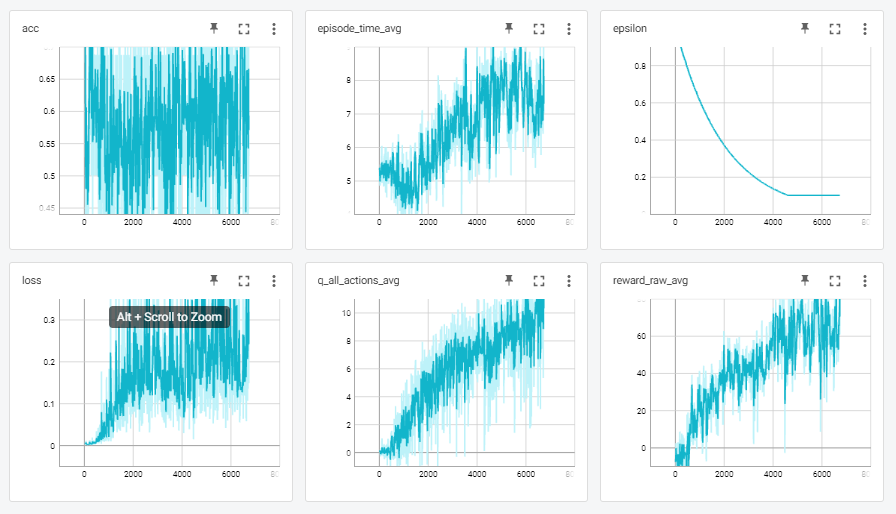
\includegraphics[width=1\linewidth]{images/tensorboard_bundaran_simpangempat_segmentasi_grayscale}
	\caption{Tensorboard pada Bundaran Simpang Empat dengan Segmentasi Grayscale}
	\label{fig:tensorboard_bundaran_simpangempat_segmentasi_grayscale}
\end{figure}

Dari hasil visualisasi \textit{training} DQN pada bundaran simpang empat dengan segmentasi grayscale pada Gambar \ref{fig:tensorboard_bundaran_simpangempat_segmentasi_grayscale}, dapat dilihat bahwa proses \textit{training} algoritma DQN telah berjalan dengan baik. Hal itu dapat dilihat dari nilai akurasi, \textit{episode time}, dan \textit{reward} berkendara mobil otonom yang mengalami tren kenaikan seiring dengan berjalannya proses training.

\subsection{\textit{Training} DQN pada Bundaran Simpang Empat dengan Segmentasi Lanjutan}
\label{sec:training_dqn_bundaran_simpangempat_segmentasi_hitam_putih}

\textit{Training} algoritma DQN pada bundaran simpang empat dengan segmentasi lanjutan berlangsung selama 13 jam, 30 menit, dan 48 detik. Visualisasi \textit{training} algoritma DQN dapat dilihat pada Gambar \ref{fig:tensorboard_bundaran_simpangempat_segmentasi_lanjutan}.

\begin{figure}[H] 
	\centering
	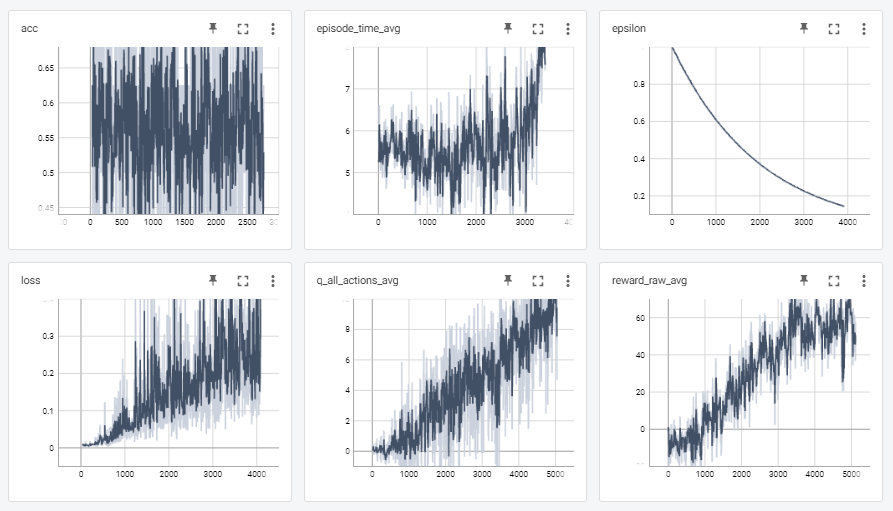
\includegraphics[width=1\linewidth]{images/tensorboard_bunderan_segmented}
	\caption{Tensorboard pada Bundaran Simpang Empat dengan Segmentasi Lanjutan}
	\label{fig:tensorboard_bundaran_simpangempat_segmentasi_lanjutan}
\end{figure}

Dari hasil visualisasi \textit{training} DQN pada bundaran simpang empat dengan segmentasi lanjutan pada Gambar \ref{fig:tensorboard_bundaran_tanpasimpang_segmentasi_lanjutan}, dapat dilihat bahwa proses \textit{training} algoritma DQN telah berjalan dengan baik. Hal itu dapat dilihat dari nilai akurasi, \textit{episode time}, dan \textit{reward} berkendara mobil otonom yang mengalami tren kenaikan seiring dengan berjalannya proses \textit{training}.


\subsection{\textit{Training} DQN pada Bundaran Tanpa Simpang dengan Segmentasi Lanjutan}
\label{sec:training_dqn_bundaran_nosimpang_segmentasi_hitam_putih}

\textit{Training} algoritma DQN pada bundaran tanpa simpang dengan segmentasi lanjutan berlangsung selama 26 jam dan 25 detik. Visualisasi \textit{training} algoritma DQN dapat dilihat pada Gambar \ref{fig:tensorboard_bundaran_tanpasimpang_segmentasi_lanjutan}.

\begin{figure}[H] 
	\centering
	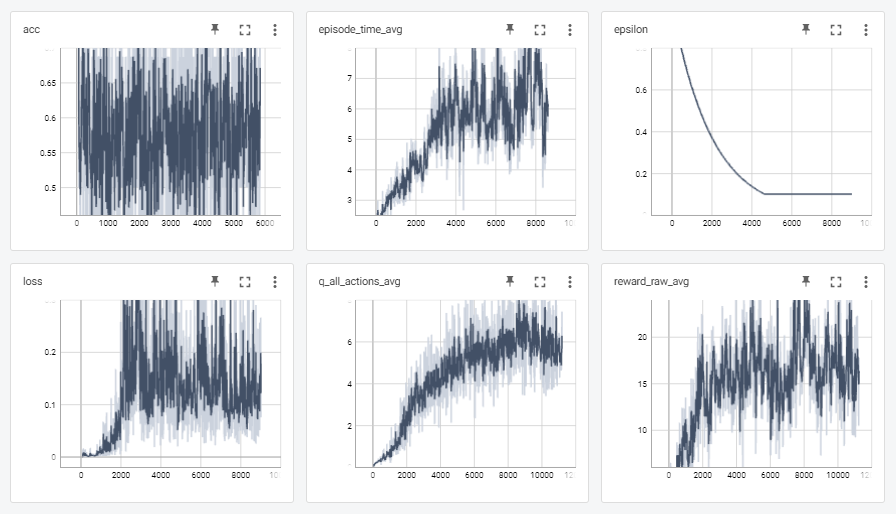
\includegraphics[width=1\linewidth]{images/tensorboard_itemputih_nosimpang}
	\caption{Tensorboard pada Bundaran Tanpa Simpang dengan Segmentasi Lanjutan}
	\label{fig:tensorboard_bundaran_tanpasimpang_segmentasi_lanjutan}
\end{figure}

Dari hasil visualisasi \textit{training} DQN pada bundaran tanpa simpang dengan segmentasi lanjutan pada Gambar \ref{fig:tensorboard_bundaran_tanpasimpang_segmentasi_lanjutan}, dapat dilihat bahwa proses \textit{training} algoritma DQN telah berjalan dengan baik. Hal itu dapat dilihat dari nilai akurasi, \textit{episode time}, dan \textit{reward} berkendara mobil otonom yang mengalami tren kenaikan seiring dengan berjalannya proses training.


\iffalse
Training algoritma DQN dengan
berlangsung selama 81 jam, 12 menit, dan 38 detik. Berikut adalah hasil visualisasi training algoritma DQN:

\begin{figure}[H] 
	\centering
	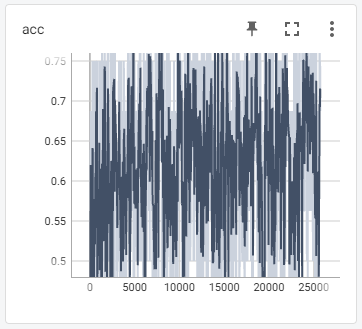
\includegraphics[width=.7\linewidth]{images/acc}
	\caption{Nilai akurasi}
	\label{fig:acc}
\end{figure}
\begin{figure}[H] 
	\centering
	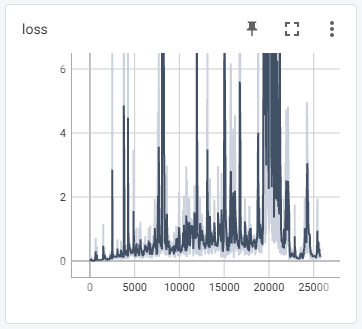
\includegraphics[width=.7\linewidth]{images/loss}
	\caption{Nilai loss}
	\label{fig:loss}
\end{figure}
\begin{figure}[H] 
	\centering
	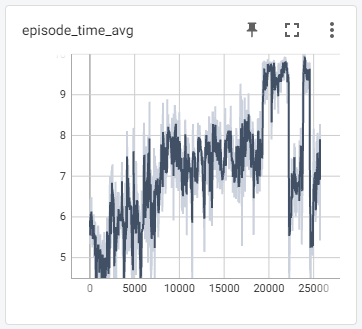
\includegraphics[width=.7\linewidth]{images/episode_time_avg}
	\caption{Rerata waktu episode}
	\label{fig:episode_time_avg}
\end{figure}
\begin{figure}[H] 
	\centering
	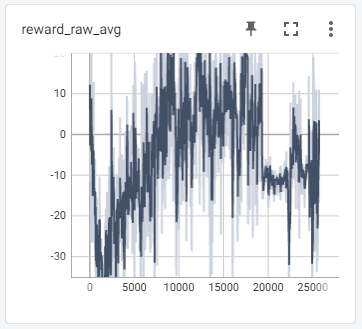
\includegraphics[width=.7\linewidth]{images/reward_raw_avg}
	\caption{Rerata nilai reward \textit{raw}}
	\label{fig:reward_raw_avg}
\end{figure}
\begin{figure}[H] 
	\centering
	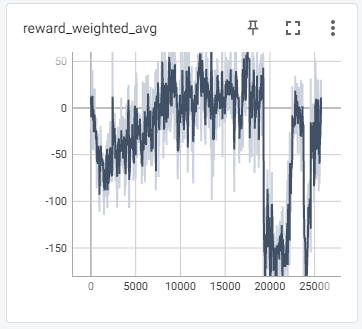
\includegraphics[width=.7\linewidth]{images/reward_weighted_avg}
	\caption{Rerata nilai reward \textit{weighted}}
	\label{fig:reward_weighted_avg}
\end{figure}
\begin{figure}[H] 
	\centering
	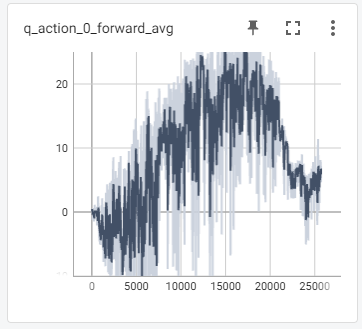
\includegraphics[width=.7\linewidth]{images/q_action_0_forward_avg}
	\caption{Nilai rerata q dari action forward}
	\label{fig:q_action_0_forward_avg}
\end{figure}
\begin{figure}[H] 
	\centering
	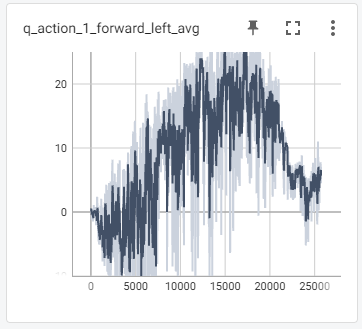
\includegraphics[width=.7\linewidth]{images/q_action_1_forward_left_avg}
	\caption{Nilai rerata q dari action forward left}
	\label{fig:q_action_1_forward_left_avg}
\end{figure}
\begin{figure}[H] 
	\centering
	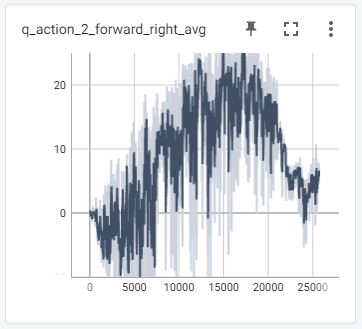
\includegraphics[width=.7\linewidth]{images/q_action_2_forward_right_avg}
	\caption{Nilai rerata q dari action forward right}
	\label{fig:q_action_2_forward_right_avg}
\end{figure}
\begin{figure}[H] 
	\centering
	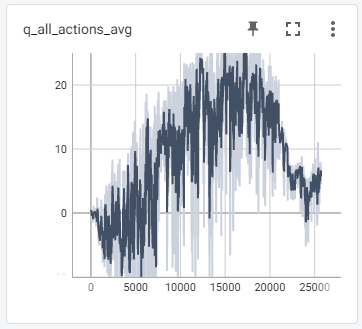
\includegraphics[width=.7\linewidth]{images/q_all_actions_avg}
	\caption{Nilai rerata q dari seluruh action}
	\label{fig:q_all_actions_avg}
\end{figure}

Dari hasil visualisasi training DQN diatas, dapat dilihat bahwa proses training algoritma DQN telah berjalan dengan baik. Hal itu dapat dilihat dari nilai akurasi, \textit{episode time}, dan \textit{reward} berkendara mobil otonom yang mengalami tren kenaikan seiring dengan berjalannya proses training.

\fi

\section{Pengujian Model DQN}
\label{sec:pengujian_model_dqn}

Pada bagian ini, dilakukan pengujian model hasil dari proses \textit{training} model DQN.

\subsection{Pengujian Model DQN pada Bundaran Simpang Empat dengan Segmentasi Grayscale}
\label{sec:pengujian_dqn_bundaran_simpangempat_segmentasi_grayscale}

Dilakukan pengujian perlakuan sebanyak 30 kali pemutaran episode. Dari pengujian ini didapatkan \textit{episode\_length }sebagai panjang lamanya episode, kemudian \textit{speed} sebagai kecepatan rata-rata \textit{agent} dalam kilometer per jam, kemudian \textit{angle\_diff} sebagai rata-rata deviasi sudut \textit{agent} terhadap \textit{target lane}, kemudian \textit{dist\_diff} sebagai rata-rata deviasi jarak \textit{agent} terhadap target\_lane, serta \textit{reward} sebagai rata-rata \textit{reward }\textit{agent} tersebut setiap episodenya. Hasil pengujian dapat dilihat pada Tabel \ref{tb:hasilpengujian_bunderan_grayscale}.

\iffalse
Dari hasil yang terlihat pada Tabel \ref{tb:hasilpengujian_bunderan_grayscale} didapatkan bahwa masih terdapat fluktuasi pada \textit{episode\_length} dan terlihat bahwa model belum konvergen.
\fi

% Please add the following required packages to your document preamble:
% \usepackage{graphicx}
\begin{table}[H]
	\resizebox{\textwidth}{!}{%
		\begin{tabular}{|r|r|r|r|r|r|}
			\hline
			\multicolumn{1}{|l|}{nomor} &
			\multicolumn{1}{l|}{episode\_length} &
			\multicolumn{1}{l|}{speed} &
			\multicolumn{1}{l|}{angle\_diff} &
			\multicolumn{1}{l|}{dist\_diff} &
			\multicolumn{1}{l|}{reward} \\ \hline
			1  & 9.005  & 34.983 & 20.001 & 5.812  & 0.166  \\ \hline
			2  & 4.772  & 28.927 & 12.140 & 0.910  & 0.448  \\ \hline
			3  & 8.524  & 33.052 & 10.650 & 1.993  & 0.398  \\ \hline
			4  & 12.678 & 35.053 & 15.259 & 3.264  & 0.222  \\ \hline
			5  & 13.621 & 37.030 & 32.642 & 12.394 & 0.122  \\ \hline
			6  & 4.851  & 30.102 & 10.241 & 1.253  & 0.471  \\ \hline
			7  & 6.555  & 20.433 & 21.370 & 2.775  & 0.318  \\ \hline
			8  & 8.694  & 31.494 & 14.927 & 3.381  & 0.235  \\ \hline
			9  & 20.184 & 34.142 & 58.799 & 45.228 & -0.230 \\ \hline
			10 & 10.026 & 28.305 & 12.737 & 2.411  & 0.332  \\ \hline
			11 & 5.147  & 29.648 & 17.682 & 1.707  & 0.289  \\ \hline
			12 & 8.521  & 32.238 & 13.255 & 2.253  & 0.289  \\ \hline
			13 & 7.990  & 32.617 & 13.939 & 2.661  & 0.342  \\ \hline
			14 & 5.206  & 30.142 & 13.541 & 1.077  & 0.409  \\ \hline
			15 & 6.072  & 23.770 & 36.641 & 3.617  & 0.170  \\ \hline
			16 & 5.426  & 31.166 & 12.926 & 0.925  & 0.418  \\ \hline
			17 & 5.176  & 27.477 & 12.276 & 1.194  & 0.457  \\ \hline
			18 & 8.085  & 33.884 & 11.883 & 1.224  & 0.343  \\ \hline
			19 & 10.048 & 27.918 & 15.146 & 3.086  & 0.306  \\ \hline
			20 & 7.443  & 33.063 & 12.290 & 2.298  & 0.383  \\ \hline
			21 & 29.772 & 38.947 & 65.564 & 58.657 & -0.255 \\ \hline
			22 & 6.617  & 30.019 & 20.405 & 1.658  & 0.425  \\ \hline
			23 & 4.931  & 27.362 & 12.078 & 1.821  & 0.361  \\ \hline
			24 & 14.428 & 29.973 & 18.900 & 3.066  & 0.272  \\ \hline
			25 & 5.445  & 30.364 & 10.480 & 0.951  & 0.523  \\ \hline
			26 & 8.794  & 31.964 & 15.540 & 2.635  & 0.294  \\ \hline
			27 & 8.568  & 33.002 & 13.103 & 1.950  & 0.409  \\ \hline
			28 & 20.471 & 24.614 & 64.263 & 15.817 & -0.076 \\ \hline
			29 & 5.276  & 31.540 & 14.182 & 1.594  & 0.349  \\ \hline
			30 & 7.645  & 29.516 & 39.559 & 1.573  & 0.349  \\ \hline
		\end{tabular}%
	}
	\caption{30 Sampel Hasil Model DQN pada Bundaran Simpang Empat dengan Segmentasi Grayscale.}
	\label{tb:hasilpengujian_bunderan_grayscale}
\end{table}


Dari hasil pengambilan sampel tersebut didapatkan kesimpulan seperti pada tabel \ref{tb:kesimpulan_bunderan_grayscale}.

% Please add the following required packages to your document preamble:
% \usepackage{graphicx}
\begin{table}[H]
	\resizebox{\textwidth}{!}{%
		\begin{tabular}{|l|l|l|l|l|}
			\hline
			avg\_episode\_length & avg\_speed & avg\_angle\_diff & avg\_dist\_diff & avg\_reward \\ \hline
			9.332                & 30.758     & 21.413           & 6.306           & 0.284       \\ \hline
		\end{tabular}%
	}
	\caption{Kesimpulan Hasil Model DQN pada Bundaran Simpang Empat dengan Segmentasi Grayscale.}
	\label{tb:kesimpulan_bunderan_grayscale}
\end{table}



\subsection{Pengujian Model DQN pada Bundaran Simpang Empat dengan Segmentasi Lanjutan}
\label{sec:pengujian_dqn_bundaran_simpangempat_segmentasi_hitam_putih}

Dilakukan pengujian perlakuan sebanyak 30 kali pemutaran episode. Dari pengujian ini didapatkan \textit{episode\_length }sebagai panjang lamanya episode, kemudian \textit{speed} sebagai kecepatan rata-rata \textit{agent} dalam kilometer per jam, kemudian \textit{angle\_diff} sebagai rata-rata deviasi sudut \textit{agent} terhadap \textit{target lane}, kemudian \textit{dist\_diff} sebagai rata-rata deviasi jarak \textit{agent} terhadap target\_lane, serta \textit{reward} sebagai rata-rata \textit{reward }\textit{agent} tersebut setiap episodenya. Hasil pengujian dapat dilihat pada Tabel \ref{tb:hasilpengujian_bunderan_segmented}.

% Please add the following required packages to your document preamble:
% \usepackage{graphicx}
\begin{table}[H]
	\resizebox{\textwidth}{!}{%
		\begin{tabular}{|r|r|r|r|r|r|}
			\hline
			\multicolumn{1}{|l|}{nomor} &
			\multicolumn{1}{l|}{episode\_length} &
			\multicolumn{1}{l|}{speed} &
			\multicolumn{1}{l|}{angle\_diff} &
			\multicolumn{1}{l|}{dist\_diff} &
			\multicolumn{1}{l|}{reward} \\ \hline
			1  & 7.431  & 38.229 & 10.205 & 2.000  & 0.340  \\ \hline
			2  & 8.094  & 30.830 & 24.743 & 1.187  & 0.392  \\ \hline
			3  & 8.418  & 30.337 & 20.039 & 2.106  & 0.257  \\ \hline
			4  & 21.587 & 37.044 & 14.712 & 2.588  & 0.280  \\ \hline
			5  & 7.019  & 35.495 & 11.015 & 0.849  & 0.465  \\ \hline
			6  & 19.252 & 35.029 & 20.848 & 3.259  & 0.267  \\ \hline
			7  & 18.607 & 29.382 & 58.620 & 6.881  & 0.071  \\ \hline
			8  & 6.529  & 36.715 & 10.400 & 1.301  & 0.348  \\ \hline
			9  & 14.337 & 36.066 & 16.105 & 0.990  & 0.421  \\ \hline
			10 & 17.025 & 34.249 & 45.883 & 4.252  & 0.150  \\ \hline
			11 & 9.511  & 41.363 & 12.647 & 1.503  & 0.320  \\ \hline
			12 & 36.864 & 34.917 & 68.418 & 8.128  & 0.069  \\ \hline
			13 & 9.973  & 38.902 & 13.901 & 1.560  & 0.304  \\ \hline
			14 & 7.340  & 35.594 & 13.333 & 1.547  & 0.450  \\ \hline
			15 & 14.864 & 31.482 & 59.456 & 3.588  & 0.112  \\ \hline
			16 & 9.987  & 41.680 & 12.595 & 1.952  & 0.297  \\ \hline
			17 & 9.767  & 39.018 & 15.001 & 1.341  & 0.373  \\ \hline
			18 & 7.011  & 36.749 & 10.620 & 1.488  & 0.321  \\ \hline
			19 & 17.400 & 26.631 & 79.254 & 13.336 & -0.070 \\ \hline
			20 & 12.798 & 40.187 & 15.749 & 1.645  & 0.285  \\ \hline
			21 & 17.809 & 31.448 & 46.125 & 2.951  & 0.268  \\ \hline
			22 & 11.504 & 36.149 & 21.827 & 1.347  & 0.355  \\ \hline
			23 & 6.395  & 37.127 & 9.601  & 0.895  & 0.418  \\ \hline
			24 & 23.591 & 30.945 & 60.991 & 4.070  & 0.153  \\ \hline
			25 & 6.957  & 37.284 & 8.505  & 0.959  & 0.438  \\ \hline
			26 & 9.431  & 40.093 & 11.436 & 1.980  & 0.311  \\ \hline
			27 & 35.604 & 27.912 & 80.507 & 11.311 & -0.171 \\ \hline
			28 & 9.089  & 42.260 & 10.891 & 1.286  & 0.395  \\ \hline
			29 & 7.032  & 36.387 & 11.418 & 1.278  & 0.418  \\ \hline
			30 & 8.578  & 34.796 & 15.489 & 1.456  & 0.316  \\ \hline
		\end{tabular}%
	}
	\caption{30 Sampel Hasil Model DQN pada Bundaran Simpang Empat dengan Segmentasi Lanjutan.}
	\label{tb:hasilpengujian_bunderan_segmented}
\end{table}


Dari hasil pengambilan sampel tersebut didapatkan kesimpulan seperti pada tabel \ref{tb:kesimpulan_bunderan_segmented}.


% Please add the following required packages to your document preamble:
% \usepackage{graphicx}
\begin{table}[H]
	\resizebox{\textwidth}{!}{%
		\begin{tabular}{|l|l|l|l|l|}
			\hline
			avg\_episode\_length & avg\_speed & avg\_angle\_diff & avg\_dist\_diff & avg\_reward \\ \hline
			13.326                & 35.476     & 27.011           & 2.967           & 0.278       \\ \hline
		\end{tabular}%
	}
	\caption{Kesimpulan Hasil Model DQN pada Bundaran Simpang Empat dengan Segmentasi Lanjutan.}
	\label{tb:kesimpulan_bunderan_segmented}
\end{table}

\subsection{Pengujian Model DQN pada Bundaran Tanpa Simpang dengan Segmentasi Lanjutan}
\label{sec:pengujian_dqn_bundaran_nosimpang_segmentasi_hitam_putih}

Dilakukan pengujian perlakuan sebanyak 30 kali pemutaran episode. Dari pengujian ini didapatkan \textit{episode\_length }sebagai panjang lamanya episode, kemudian \textit{speed} sebagai kecepatan rata-rata \textit{agent} dalam kilometer per jam, kemudian \textit{alpha} sebagai rata-rata deviasi sudut \textit{agent} terhadap \textit{waypoint} terdekat + 5, serta \textit{reward} sebagai rata-rata \textit{reward }\textit{agent} tersebut setiap episodenya. Hasil pengujian dapat dilihat pada Tabel \ref{tb:hasilpengujian_notbunderan_segmented}.

\begin{table}[H]
	\begin{tabular}{|r|r|r|r|r|}
		\hline
		\multicolumn{1}{|l|}{nomor} & \multicolumn{1}{l|}{episode\_length} & \multicolumn{1}{l|}{speed} & \multicolumn{1}{l|}{alpha} & \multicolumn{1}{l|}{reward} \\ \hline
		1  & 8.374  & 32.202 & 31.098 & 0.113 \\ \hline
		2  & 8.796  & 29.909 & 32.023 & 0.093 \\ \hline
		3  & 12.195 & 29.678 & 40.528 & 0.068 \\ \hline
		4  & 12.439 & 30.384 & 36.557 & 0.120 \\ \hline
		5  & 10.246 & 29.720 & 42.027 & 0.063 \\ \hline
		6  & 3.138  & 19.860 & 32.557 & 0.085 \\ \hline
		7  & 9.982  & 30.777 & 35.319 & 0.129 \\ \hline
		8  & 8.185  & 30.640 & 24.322 & 0.112 \\ \hline
		9  & 9.719  & 31.814 & 31.563 & 0.081 \\ \hline
		10 & 10.908 & 33.314 & 38.641 & 0.097 \\ \hline
		11 & 3.299  & 21.882 & 22.220 & 0.122 \\ \hline
		12 & 9.270  & 31.347 & 26.635 & 0.120 \\ \hline
		13 & 4.270  & 26.317 & 16.402 & 0.152 \\ \hline
		14 & 3.765  & 23.032 & 32.140 & 0.169 \\ \hline
		15 & 10.776 & 31.581 & 37.949 & 0.091 \\ \hline
		16 & 5.588  & 28.784 & 29.461 & 0.155 \\ \hline
		17 & 3.219  & 22.536 & 20.392 & 0.186 \\ \hline
		18 & 8.508  & 30.489 & 24.669 & 0.122 \\ \hline
		19 & 4.457  & 23.680 & 23.546 & 0.146 \\ \hline
		20 & 3.824  & 22.575 & 36.989 & 0.105 \\ \hline
		21 & 10.599 & 31.869 & 23.992 & 0.132 \\ \hline
		22 & 12.438 & 31.080 & 38.071 & 0.088 \\ \hline
		23 & 7.873  & 31.305 & 21.448 & 0.150 \\ \hline
		24 & 3.562  & 22.864 & 16.225 & 0.136 \\ \hline
		25 & 8.758  & 27.877 & 37.786 & 0.076 \\ \hline
		26 & 4.641  & 26.732 & 25.345 & 0.106 \\ \hline
		27 & 10.472 & 32.074 & 33.322 & 0.101 \\ \hline
		28 & 10.937 & 31.784 & 33.864 & 0.095 \\ \hline
		29 & 9.244  & 30.508 & 28.196 & 0.120 \\ \hline
		30 & 9.273  & 29.378 & 28.780 & 0.119 \\ \hline
	\end{tabular}
	\caption{30 Sampel Hasil Model DQN pada Bundaran Tanpa Simpang dengan Segmentasi Lanjutan.}
	\label{tb:hasilpengujian_notbunderan_segmented}
\end{table}

Dari hasil pengambilan sampel tersebut didapatkan kesimpulan seperti pada tabel \ref{tb:kesimpulan_notbunderan_segmented}.

% Please add the following required packages to your document preamble:
% \usepackage{graphicx}
\begin{table}[H]
	\resizebox{\textwidth}{!}{%
		\begin{tabular}{|l|l|l|l|}
			\hline
			avg\_episode\_length & avg\_speed & avg\_alpha & avg\_reward \\ \hline
			7.958                & 28.533     & 30.068     & 0.115       \\ \hline
		\end{tabular}%
	}
	\caption{Kesimpulan Hasil Model DQN pada Bundaran Tanpa Simpang dengan Segmentasi Lanjutan.}
	\label{tb:kesimpulan_notbunderan_segmented}
\end{table}


\iffalse
\subsection{Hasil Setelah Learning 12 jam}
\label{sec:hasil_learning_12}
Setelah learning selama 12 jam, didapatkan model reinforcement yang sudah cukup memahami kehadiran bundaran di depan agent. Pada salah satu run simulasi Gambar \ref{fig:uji0}, didapatkan agent yang mampu bergerak lurus ke depan hingga mendekati bundaran, dan mampu melakukan manuver kanan lalu ke kiri lagi (dan arah kembali sejajar dengan arah pada saat start) agar tidak menyentuh bundaran. Meskipun pada akhirnya agent menyentuh object rumah pada ujung jalan.

\begin{figure}[H] 
	\centering
	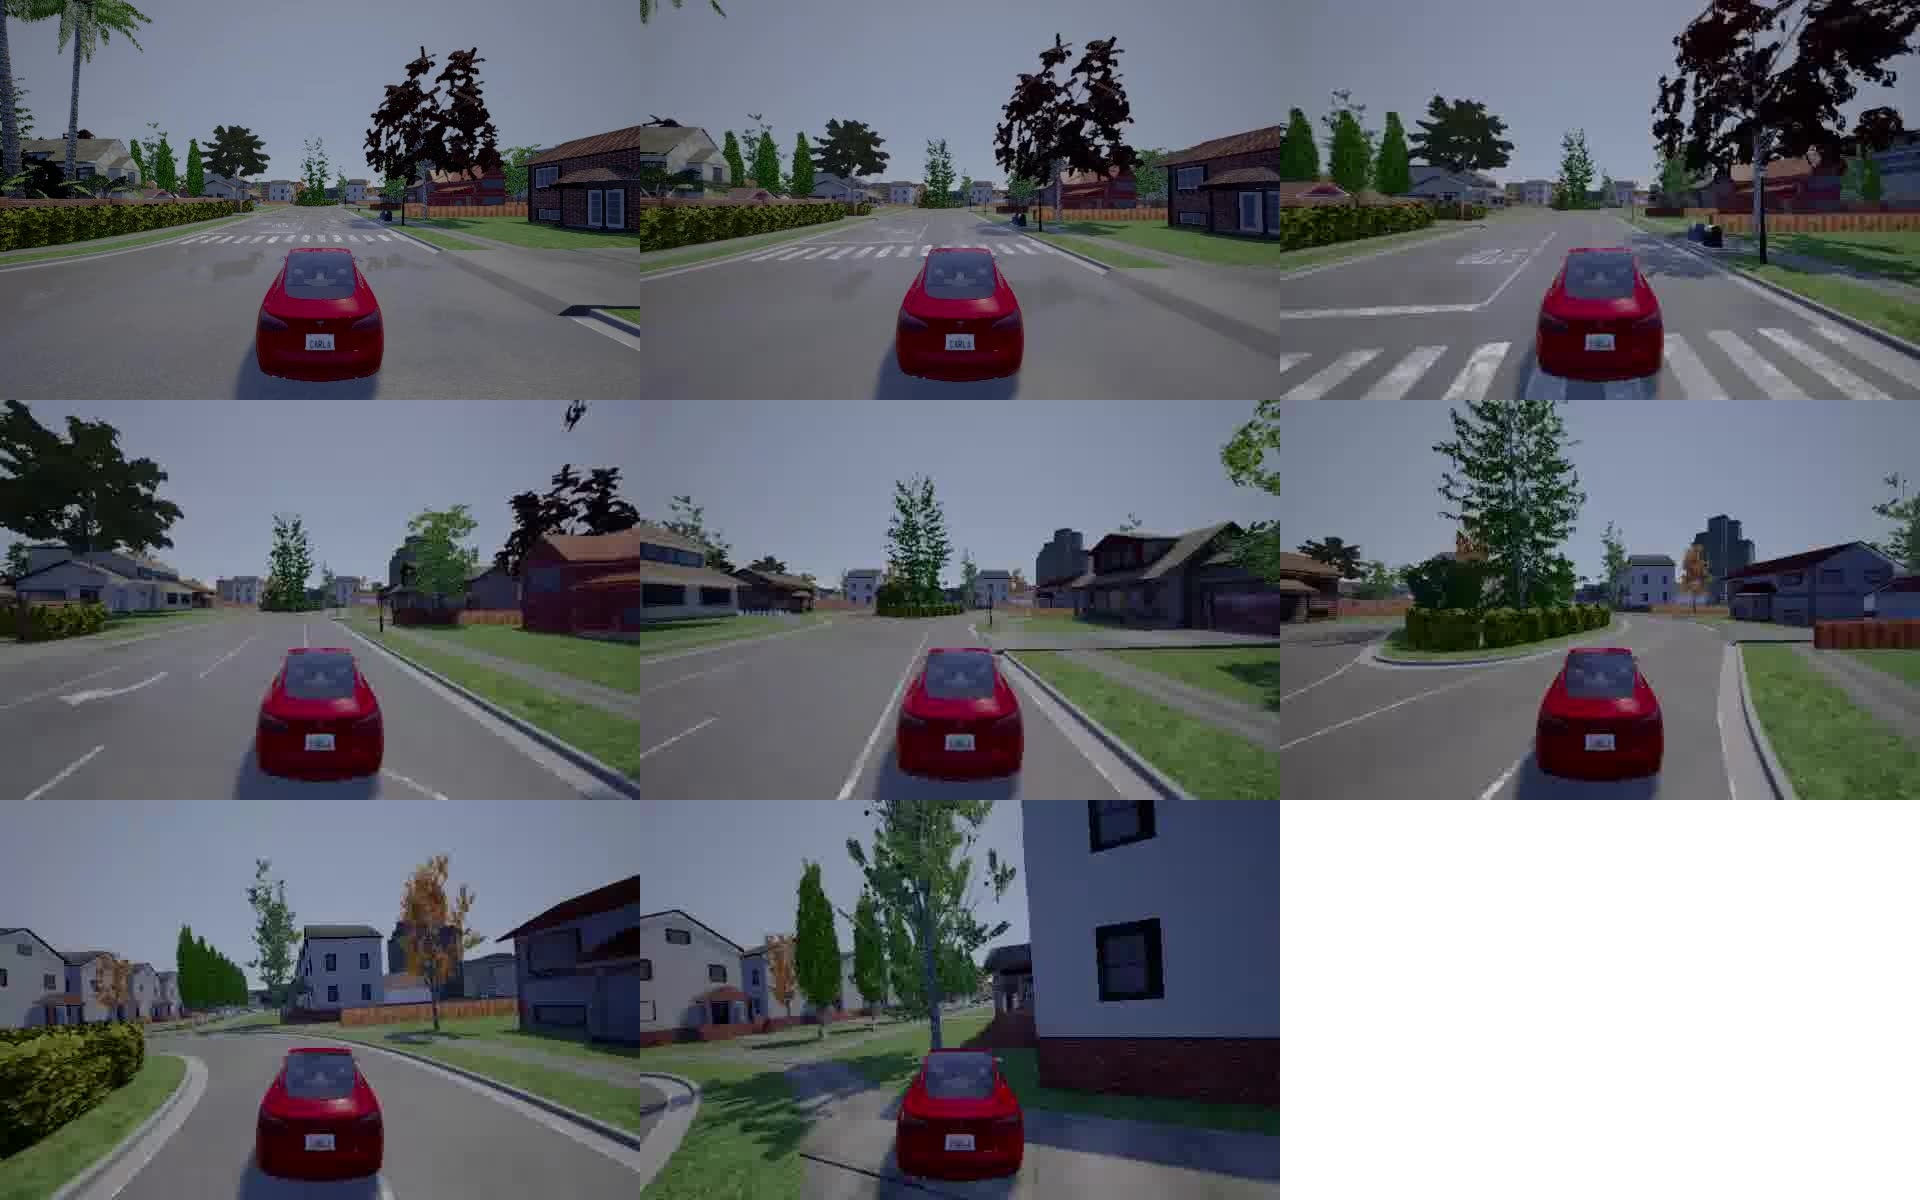
\includegraphics[width=1\linewidth]{images/uji0}
	\caption{Salah satu hasil simulasi uji. Jarak antar foto adalah 1.5 detik. Baca sekuen dari atas kiri ke kanan bawah.}
	\label{fig:uji0}
\end{figure}

\subsection{Hasil Setelah Learning 58 jam}
\label{sec:hasil_learning_12}
Setelah learning selama 58 jam, didapatkan model reinforcement yang sudah cukup memahami gerakan bahwa agent harus memutari bundaran agar mendapatkan award yang lebih besar. Pada salah satu run simulasi Gambar \ref{fig:uji1}., didapatkan agent yang mampu bergerak lurus ke depan hingga mendekati bundaran, dan mampu melakukan manuver kiri untuk menghindari bundaran, lalu melakukan manuver ke kanan mengitari bundaran dan tidak menyentuh bundaran. Meskipun pada akhirnya agent menyentuh object pagar setelah mengitari hampir 3/4 dari bundaran.
\begin{figure}[H] 
	\centering
	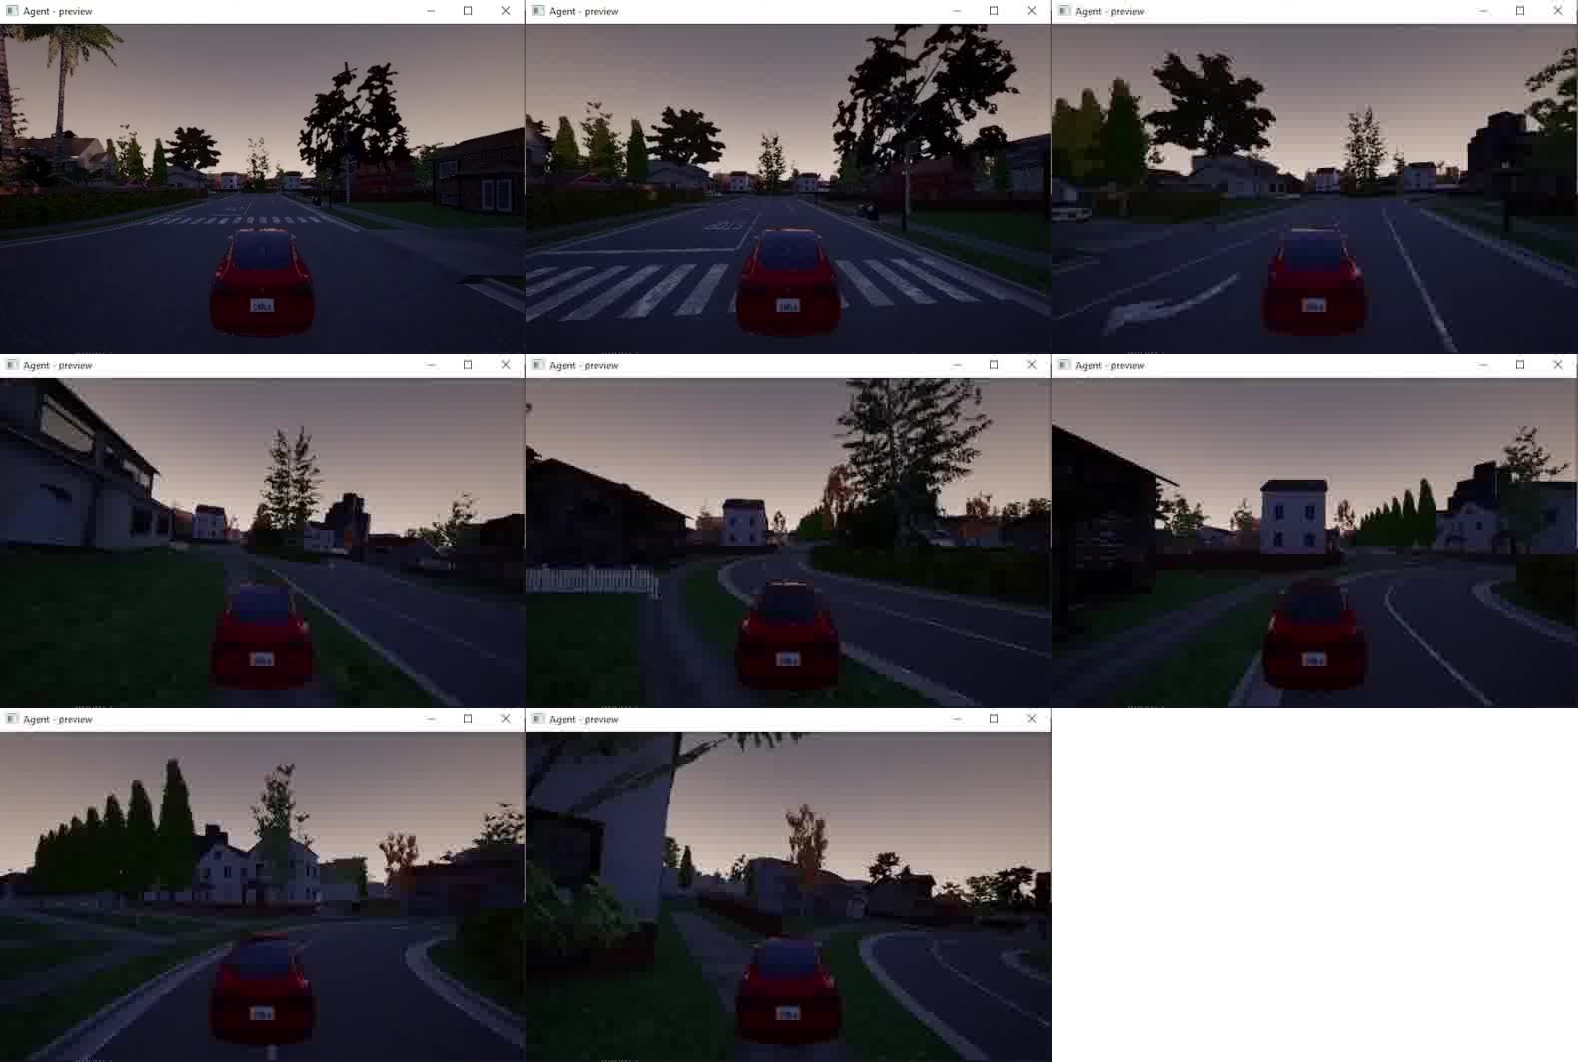
\includegraphics[width=1\linewidth]{images/uji1}
	\caption{Salah satu hasil simulasi uji. Jarak antar foto adalah 1.2 detik. Baca sekuen dari atas kiri ke kanan bawah.}
	\label{fig:uji1}
\end{figure}
\fi
